\begin{frame}
\begin{itemize}
    \item What are Multi-Layer Perceptrons
    \item Gradient Descent
    \item Code Profiling
    \item \textbf{\color{red}{CPU Parallelization}}
    \item GPU Parallelization
    \item Performance Results 
    \item Next Steps
\end{itemize}
\end{frame}

\begin{frame}
    \frametitle{CPU Optimization/Parallelization}
    \begin{itemize}
        \item Started with gpof to see what was slowing things down.
        \item Optimized serial version looking to make sure it was memory
            efficient (loops). 
        \item Found the matrix multiplication and transpose were the most heavy
            computation.
    \end{itemize}
\end{frame}

\begin{frame}
    \frametitle{Optimizing Matrix Multiplication}
    \begin{itemize}
        \item Original implementation was not great for parallelization.
        \item Introduced batching.
        \item Found that if the problem was too small parallelization made
            things worse (actually need DNN).
        \item Tried multiple versions of matrix multiply (2 naive and blocking)
    \end{itemize}
\end{frame}

\begin{frame}
    \frametitle{Performance}
    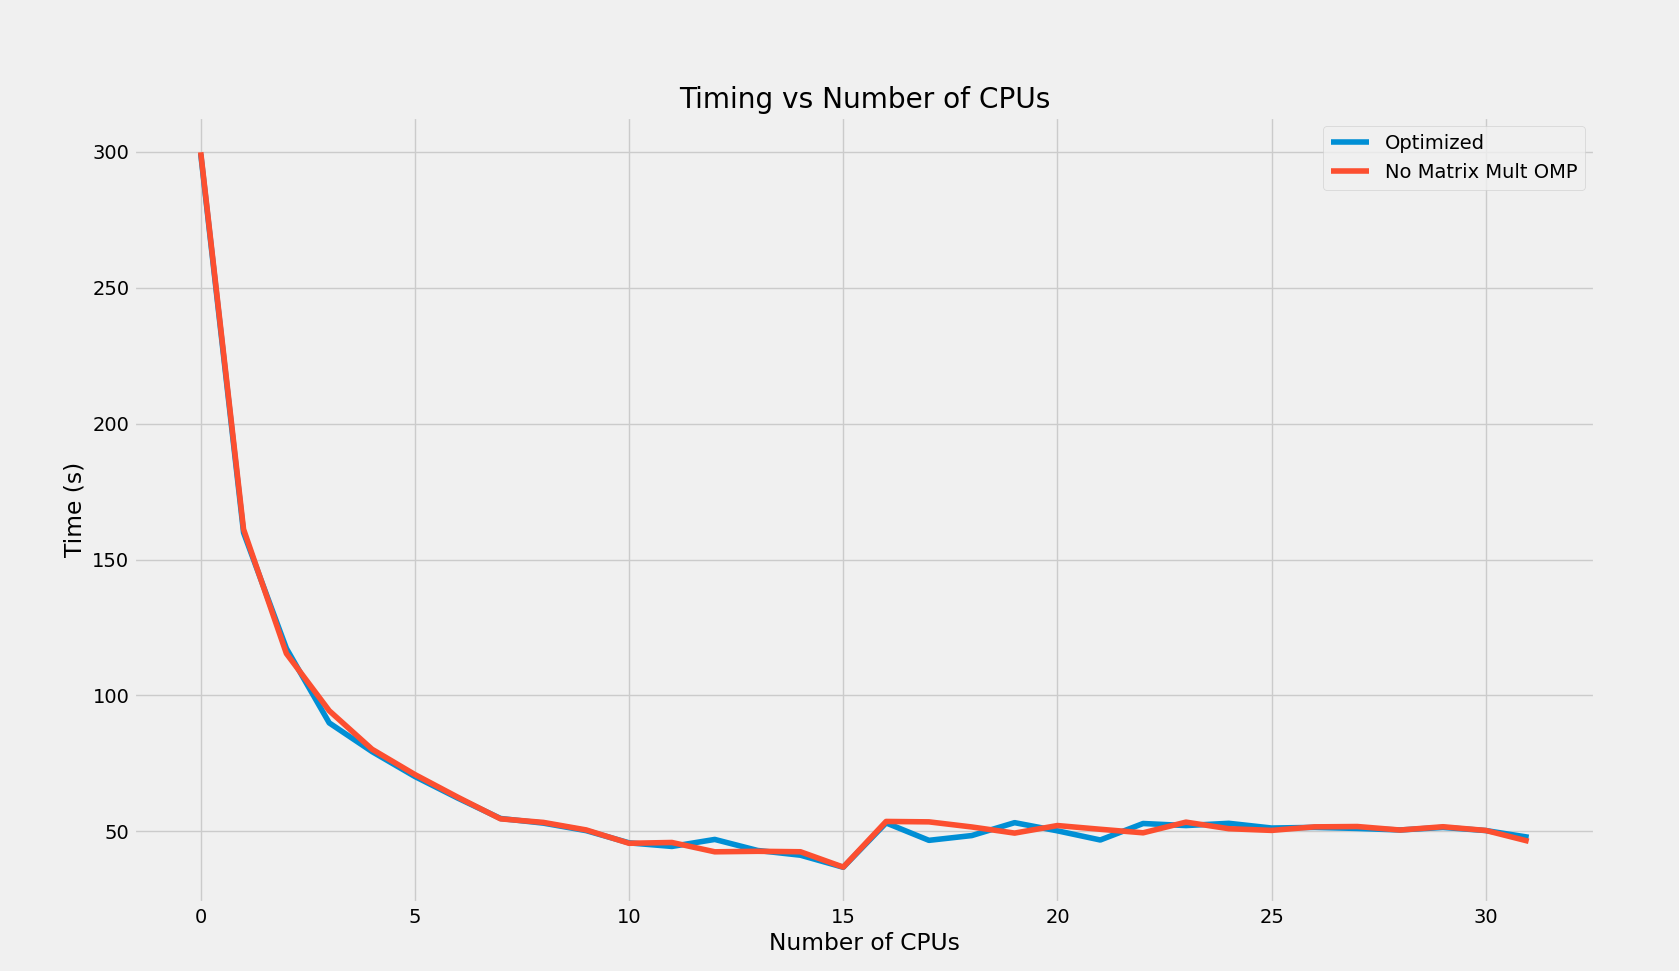
\includegraphics[width=\textwidth]{cpu.png}
\end{frame}




